\documentclass[10pt,letterpaper]{article}
\usepackage[utf8]{inputenc}
\usepackage{amsmath}
\usepackage{amsfonts}
\usepackage{amssymb}

\usepackage[margin=0.5in]{geometry}
\usepackage{graphicx}
\usepackage{tabularx}
\usepackage{booktabs}
\pagenumbering{gobble}

%compact lists
\usepackage{enumitem}
\setitemize{noitemsep,topsep=0pt,parsep=0pt,partopsep=0pt}

%fix table, figure floating issues
\usepackage[section]{placeins}

\title{Feature Testing}
\author{
	Cai, Zelin\\
	\and
	Silvestre, Patrick\\
}
\date{}

\begin{document}
\maketitle
\section{Calendar - Add Event as Student (Simplified Version)}
\subsection{Input Domain}
The input domain of this feature includes the title of the event, a date, a starting time, a ending time, a location, and a calendar. The input domain can be partitioned: e.g. one partition for title, one partition for date, etc.

\begin{figure}[h!]
	\centerline{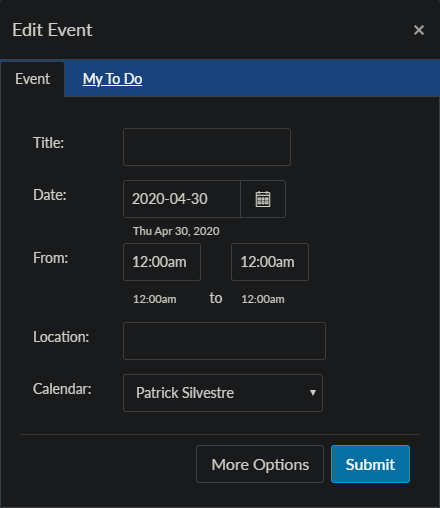
\includegraphics[width=10cm]{screenshots/edit-event.png}}
	\caption{Add Event Interface}
\end{figure}

\newpage
\subsubsection{Title}
The input domain of the input title is a string, which may be empty.

\subsubsection{Date}
The input domain of the date is a string in the format \texttt{YYYY-MM-DD}, where \texttt{YYYY} represents a year, \texttt{MM} represents a month, and \texttt{DD} represents a day. The month and day fields need not be padded with zeros. Alternatively, a user can opt to input a date using a GUI in the form of a calendar.

\subsubsection{Starting Time}
The input domain of the starting time is a string in the format \texttt{HH:MMxx}, where \texttt{HH} represents hours, \texttt{MM} represents minutes, and \texttt{xx} represents AM or PM (case insensitive). The hour and minute fields need not be padded with zeros.

\subsubsection{Ending Time}
The input domain of the ending time is a string in the format \texttt{HH:MMxx}, where \texttt{HH} represents hours, \texttt{MM} represents minutes, and \texttt{xx} represents AM or PM (case insensitive). The hour and minute fields need not be padded with zeros.

\subsubsection{Location}
The input domain of the input title is a string, which may be empty.

\subsubsection{Calendar}
The input domain of the calendar is a list of the user's calendars, of which one can be selected.

\subsection{Test Cases}
\begin{table}[!htb]
\begin{tabularx}{\textwidth}{lXXXl}
\toprule
TC \# &
  Input &
  Expected Output &
  Actual Output &
  Tess Pass/Fail \\ \midrule
1 &
  \begin{itemize}
    \item{UI: click plus (create new event) icon}
    \item{title: (empty)}
    \item{date: 2020-5-2}
    \item{starting time: 12:00am}
    \item{ending time: 12:00am}
    \item{location: (empty)}
    \item{calendar: Patrick Silvestre}
    \item{UI: click submit button}
  \end{itemize} &
  Patrick Silvestre's calendar displays Untitled event on 2020-5-2. Event has no starting nor ending time (all-day event) &
  See figure 2. &
  Pass \\ \midrule
2 &
  \begin{itemize}
    \item{UI: click plus (create new event) icon}    
    \item{title: Test}
    \item{date: 2020-5-2}
    \item{starting time: 12:00am}
    \item{ending time: 12:00am}
    \item{location: Test}
    \item{calendar: Patrick Silvestre}
    \item{UI: click submit button}
  \end{itemize} &
  Patrick Silvestre's calendar displays Test event on 2020-5-2 with Test location. Event has no starting nor ending time (all-day event). &
  See figure 3. &
  Pass \\ \bottomrule
\end{tabularx}
\end{table}

\begin{table}[!htb]
\begin{tabularx}{\textwidth}{lXXXl}
\toprule
TC \# &
  Input &
  Expected Output &
  Actual Output &
  Tess Pass/Fail \\ \midrule
3 &
  \begin{itemize}
    \item{UI: click plus (create new event) icon}
    \item{title: (empty)}
    \item{date: 2020-5-2}
    \item{starting time: 12:00pm}
    \item{ending time: 1:00pm}
    \item{location: (empty)}
    \item{calendar: Patrick Silvestre}
    \item{UI: click submit button}
  \end{itemize} &
  Patrick Silvestre's calendar displays Test event on 2020-5-2 with test location. Event has starting time 12:00pm and ending time 1:00pm). &
  See figure 4. &
  Pass \\ \midrule
4 &
  \begin{itemize}
    \item{UI: click plus (create new event) icon}
    \item{title: Test}
    \item{date: 2020-4-25}
    \item{starting time: 12:00am}
    \item{ending time: 12:00am}
    \item{location: Test}
    \item{calendar: Patrick Silvestre}
    \item{UI: click submit button}
  \end{itemize} &
  Patrick Silvestre's calendar displays Test event on 2020-4-25 with test location. Event has no starting nor ending time (all-day event). &
  See figure 5. &
  Pass \\ \midrule
5 &
  \begin{itemize}
    \item{UI: click plus (create new event) icon}
    \item{title: Test}
    \item{date: 2020-4-25}
    \item{starting time: 12:00pm}
    \item{ending time: 11:00am}
    \item{location: Test}
    \item{calendar: Patrick Silvestre}
    \item{UI: click submit button}
  \end{itemize} &
  Add Event interface warns user that event ends before it starts and prevents user from submitting event. &
  System automatically adjusts either starting or ending time to prevent invalid times with no warning, implicitly allowing user to submit event. See figure 6. &
  Fail \\ \bottomrule
\end{tabularx}
\end{table}
\FloatBarrier

\begin{figure}[!htb]
	\centerline{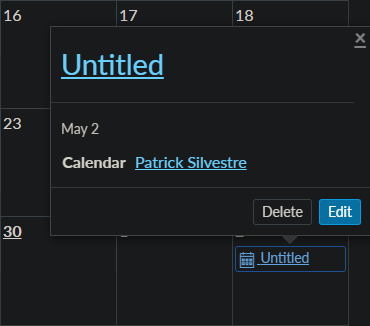
\includegraphics[]{screenshots/tc01-actual-output.png}}
	\caption{TC-01 actual output}
\end{figure}
\begin{figure}[!htb]
	\centerline{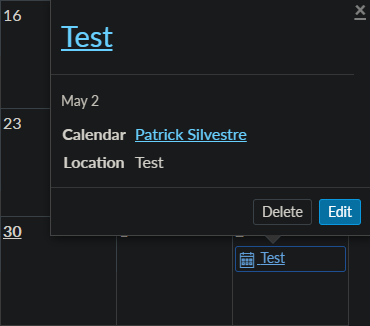
\includegraphics[]{screenshots/tc02-actual-output.png}}
	\caption{TC-02 actual output}
\end{figure}
\pagebreak
\begin{figure}[!htb]
	\centerline{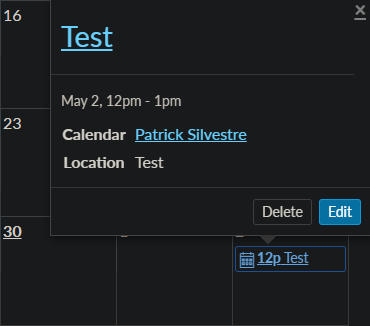
\includegraphics[]{screenshots/tc03-actual-output.png}}
	\caption{TC-03 actual output}
\end{figure}
\begin{figure}[!htb]
	\centerline{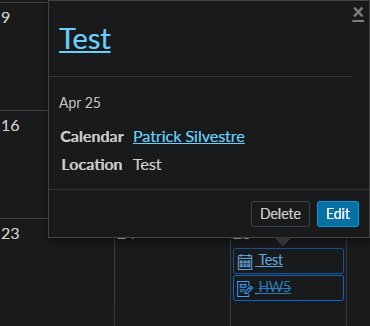
\includegraphics[]{screenshots/tc04-actual-output.png}}
	\caption{TC-04 actual output}
\end{figure}
\pagebreak
\begin{figure}[!htb]
	\centerline{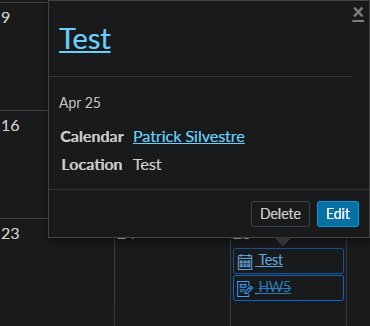
\includegraphics[]{screenshots/tc04-actual-output.png}}
	\caption{TC-04 actual output}
\end{figure}

\newpage
\section{Inbox - Composing a Message}
\subsection{Input Domain}
The input domain for the composing a message includes the Course section, the message recipients (only available after selecting the Course section), the subject of the message, the body of the message, any attachments the user wants to add to the message, and the option to send a different message to each recipient (This option will not be covered in the test cases).
Most of the input domain can be partitioned (One for the subject, one for the attachments, etc.) except for selecting the message recipient because the user must select a course before they can select their recipients.


\begin{figure}[h!]
	\centerline{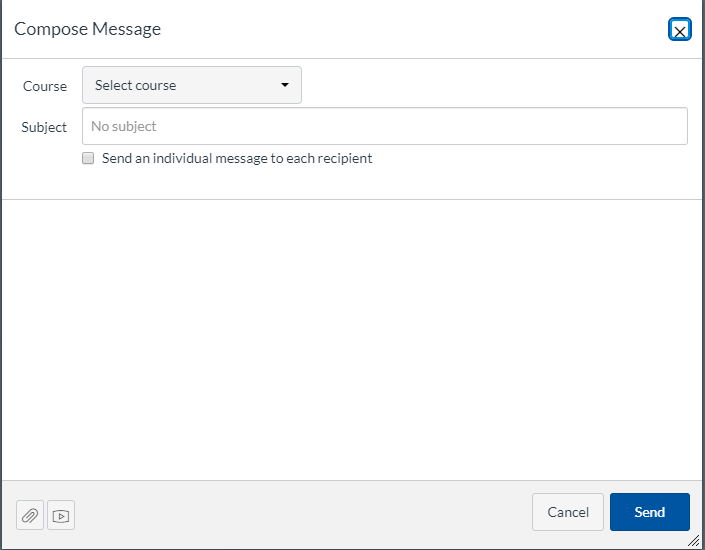
\includegraphics[width=12cm]{screenshots/compose-message-before-selecting-course.png}}
	\caption{Before selecting a course}
\end{figure}
\begin{figure}[h!]
	\centerline{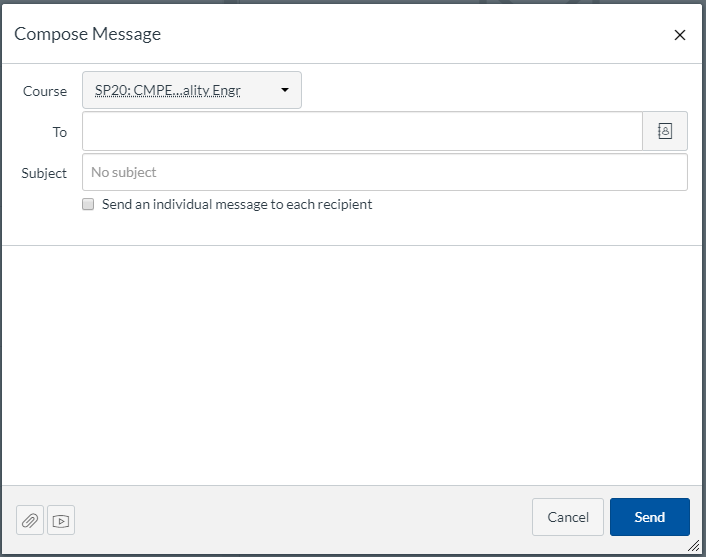
\includegraphics[width=12cm]{screenshots/compose-message-after-selecting-course.png}}
	\caption{After selecting a course}
\end{figure}
\pagebreak
\begin{figure}[h!]
	\centerline{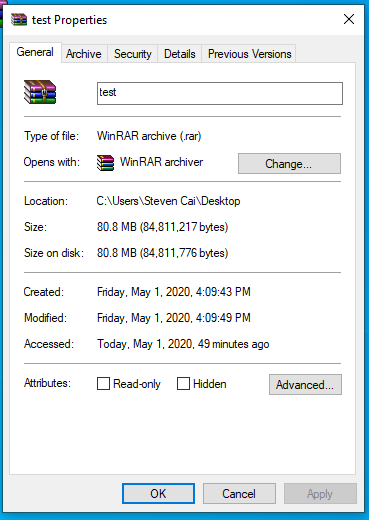
\includegraphics[width=8cm]{screenshots/compose-message-attachment.png}}
	\caption{Attachment to be used in applicable "Inbox" tests}
\end{figure}

\subsubsection{Course}
The input domain is a selection from a list of courses that the user is currently enrolled in.

\subsubsection{To}
The input domain is a selection from a list of users that are in the selected course.

\subsubsection{Subject}
The input domain is a string input.

\subsubsection{Message Body}
The input domain is a string input.

\subsubsection{Attachments}
The input domain is a file either from the user’s files on Canvas or on their computer.

\newpage
\subsection{Test Cases}
\begin{table}[h!]
\begin{tabularx}{\textwidth}{lXXXl}
\toprule
TC \# &
  Input &
  Expected Output &
  Actual Output &
  Tess Pass/Fail \\ \midrule
6 &
  \begin{itemize}
    \item{course: CMPE-187}
    \item{to: (empty)}
    \item{subject: Test1}
    \item{message: Hello there}
    \item{attachments: (empty)}
  \end{itemize} &
   Canvas informs user that recipient is invalid. &
   See figure 10. &
   Pass \\ \midrule
7 &
  \begin{itemize}
    \item{course: CMPE-187}
    \item{to: Zelin Cai}
    \item{subject: Test2}
    \item{message: (empty)}
    \item{attachments: (empty)}
  \end{itemize} &
   Canvas sends the message normally &
   See figure 11. &
   Fail \\ \midrule
8 &
  \begin{itemize}
    \item{course: CMPE-187}
    \item{to: Zelin Cai}
    \item{subject: (empty)}
    \item{message: Test Case 3}
    \item{attachments: (empty)}
  \end{itemize} &
   Canvas sends the message normally &
   Canvas outputs message title "(No Title)". See figure 12. &
   Pass \\ \midrule
9 &
  \begin{itemize}
    \item{course: CMPE-187}
    \item{to: Zelin Cai}
    \item{subject: Test4}
    \item{message: Testing Case 4}
    \item{attachments: A \texttt{.rar} file, approximately 80MB}
  \end{itemize} &
   Canvas informs the user that the file is too large for attachment. &
   Canvas sends message after about 10 minutes. See figure 13. &
   Fail \\ \midrule
10 &
  \begin{itemize}
    \item{course: (empty)}
    \item{to: (empty)}
    \item{subject: Test5}
    \item{message: Testing Case 5}
    \item{attachments: (empty)}
  \end{itemize} &
   Canvas informs user that the course selection is invalid. &
   Canvas output is identical to TC-06. See figure 14. &
   Fail \\ \bottomrule
\end{tabularx}
\end{table}

\newpage
\begin{figure}[h!]
	\centerline{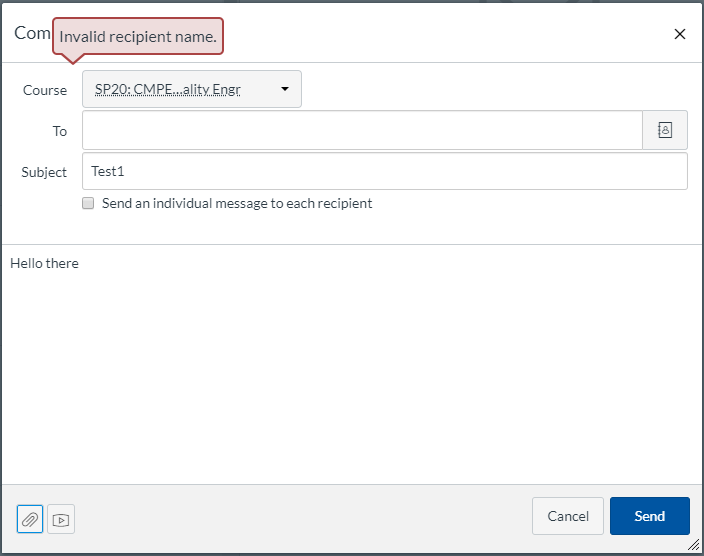
\includegraphics[width=12cm]{screenshots/tc06-actual-output.png}}
	\caption{TC-06 actual output}
\end{figure}
\begin{figure}[h!]
	\centerline{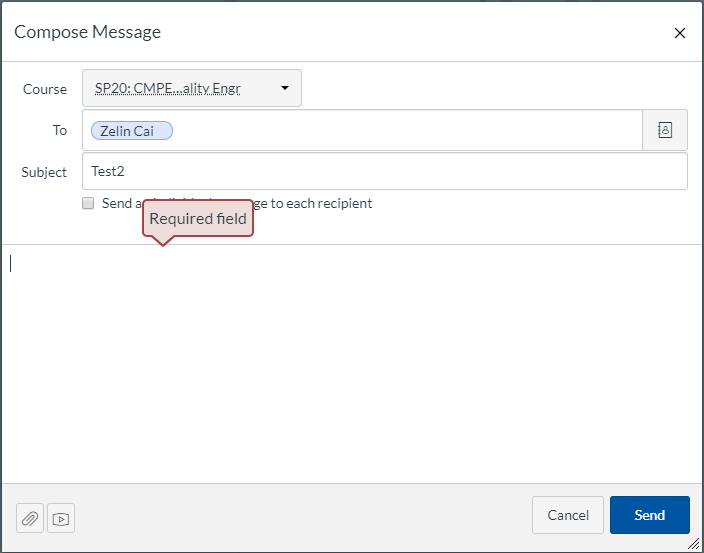
\includegraphics[width=12cm]{screenshots/tc07-actual-output.png}}
	\caption{TC-07 actual output}
\end{figure}
\pagebreak
\begin{figure}[h!]
	\centerline{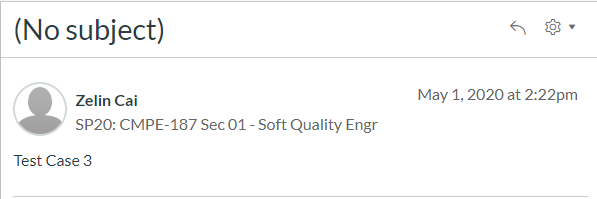
\includegraphics[width=12cm]{screenshots/tc08-actual-output.png}}
	\caption{TC-08 actual output}
\end{figure}
\begin{figure}[h!]
	\centerline{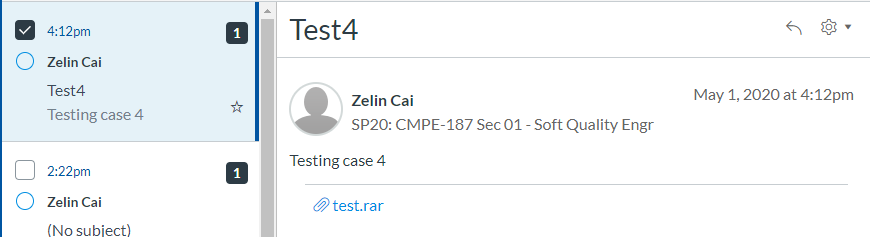
\includegraphics[width=12cm]{screenshots/tc09-actual-output.png}}
	\caption{TC-09 actual output}
\end{figure}
\begin{figure}[h!]
	\centerline{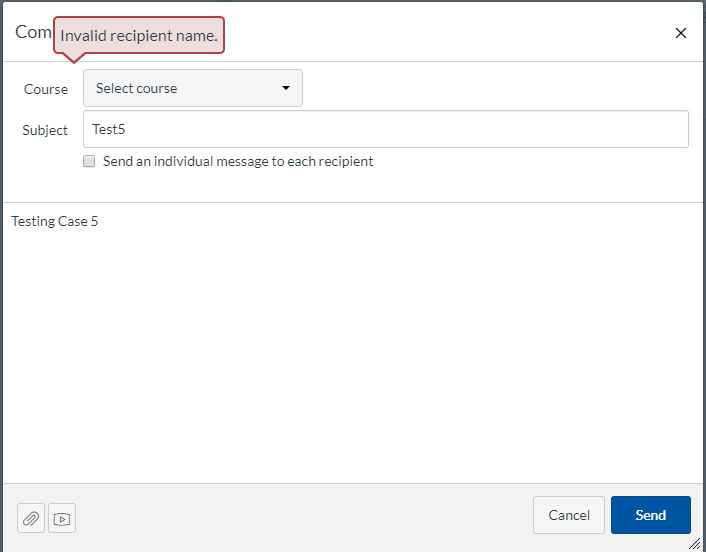
\includegraphics[width=12cm]{screenshots/tc10-actual-output.png}}
	\caption{TC-10 actual output}
\end{figure}

\newpage
\section{ePortfolios - ePortfolio Management}
\subsection{Input Domain}
The test cases will focus on creating and managing pages in an ePortfolio. This gives us a bigger input since creating a portfolio and a page in a portfolio take different inputs. The input domain for making a new ePortfolio online consists of the ePortfolio name and an option to make it public or not. When managing an ePortfolio page, the input domain includes the page name, rich text, \texttt{HTML}/embedded content, course submission (not testing this), image/file upload and the body for each of these inputs except image/file upload.

\begin{figure}[h!]
	\centerline{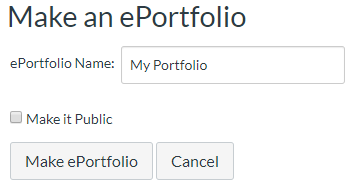
\includegraphics[width=8cm]{screenshots/create-eportfolio.png}}
	\caption{Creating an ePortfolio}
\end{figure}
\begin{figure}[h!]
	\centerline{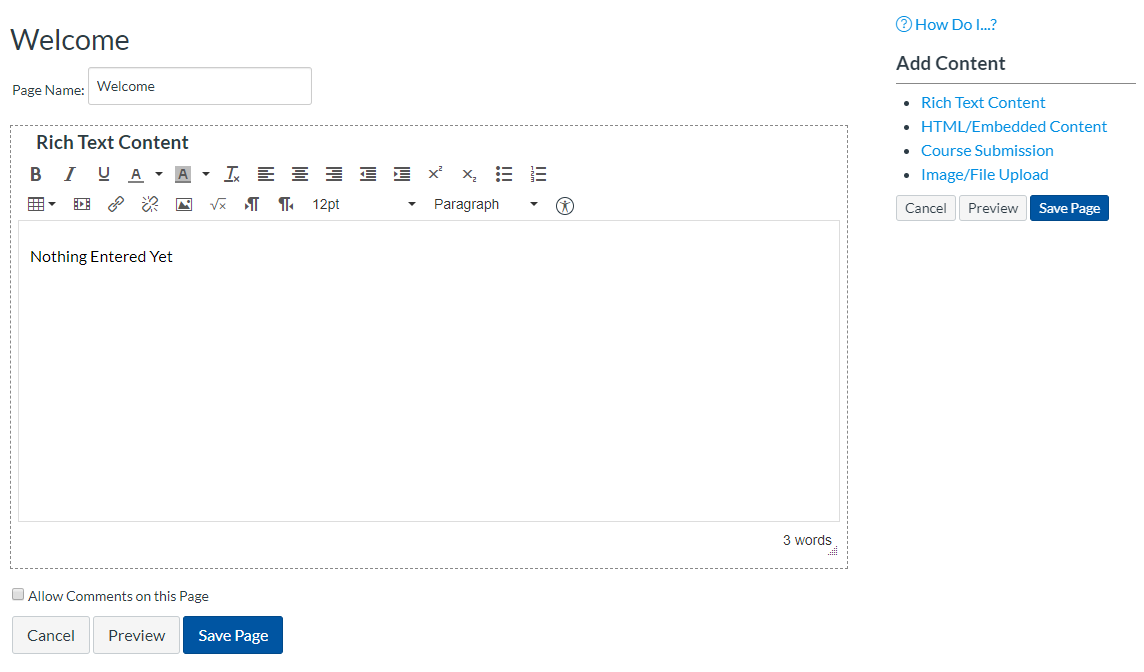
\includegraphics[width=12cm]{screenshots/create-eportfolio-page.png}}
	\caption{Creating a page inside an ePortfolio}
\end{figure}

\newpage
\subsubsection{ePortfolio Name}
The input domain is a string input.

\subsubsection{Page Name}
The input domain is a string input.

\subsubsection{Rich Text}
The input domain is a string input.

\subsubsection{\texttt{HTML}/Embedded}
The input domain is \texttt{HTML} markup or a similar markup language.

\subsubsection{Image/File}
The input domain is either an image or a file from the user's files or computer.

\subsection{Test Cases}
\begin{table}[h!]
\begin{tabularx}{\textwidth}{lXXXl}
\toprule
TC \# &
  Input &
  Expected Output &
  Actual Output &
  Tess Pass/Fail \\ \midrule
11 &
  \begin{itemize}
    \item{ePortfolio-name: (empty)}
    \item{page name: (n/a)}
    \item{rich text: (n/a)}
    \item{\texttt{HTML}/embedded: (n/a)}
    \item{image/file: (n/a)}
  \end{itemize} &
   Canvas does not create ePortfolio. &
   See figure 17. &
   Pass \\ \midrule
12 &
  \begin{itemize}
    \item{ePortfolio-name: test}
    \item{page name: (empty)}
    \item{rich text: Testing Case 2}
    \item{\texttt{HTML}/embedded: (empty)}
    \item{image/file: (empty)}
  \end{itemize} &
   Canvas notifies user a page title is required. &
   Canvas creates the page with no warnings. See figure 18. &
   Fail \\ \midrule
13 &
  \begin{itemize}
    \item{ePortfolio-name: test}
    \item{page name: Testing Case 3}
    \item{rich text: (empty)}
    \item{\texttt{HTML}/embedded: (empty)}
    \item{image/file: (empty)}
  \end{itemize} &
   Canvas creates the page, displaying only the title. &
   Leaving text blank reverts it to its previous text. See figure 19. &
   Fail \\ \bottomrule
\end{tabularx}
\end{table}



\begin{table}[h!]
\begin{tabularx}{\textwidth}{lXXXl}
\toprule
TC \# &
  Input &
  Expected Output &
  Actual Output &
  Tess Pass/Fail \\ \midrule
14 &
  \begin{itemize}
    \item{ePortfolio-name: test}
    \item{page name: Testing Case 4}
    \item{rich text: (empty)}
    \item{\texttt{HTML}/embedded: "Definitely not HTML code."}
    \item{image/file: (empty)}
  \end{itemize} &
   Canvas displays nothing (invalid HTML code). &
   Canvas treats input as rich text. See figure 20. &
   Fail \\ \midrule
15 &
  \begin{itemize}
    \item{ePortfolio-name: test}
    \item{page name: Testing Case 5}
    \item{rich text: (empty)}
    \item{\texttt{HTML}/embedded: (empty)}
    \item{image/file: A \texttt{.rar} file, approximately 80 MB.}
  \end{itemize} &
   Canvas informs the user that the file is too large for upload. &
   Canvas uploads the file after a few minutes. Upload duration was shorter than TC-09. See figure 21. &
   Fail \\ \bottomrule
\end{tabularx}
\end{table}

\newpage
\begin{figure}[h!]
	\centerline{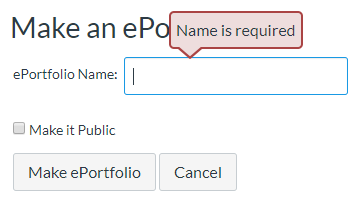
\includegraphics[width=8cm]{screenshots/tc11-actual-output.png}}
	\caption{TC-11 actual output}
\end{figure}
\begin{figure}[h!]
	\centerline{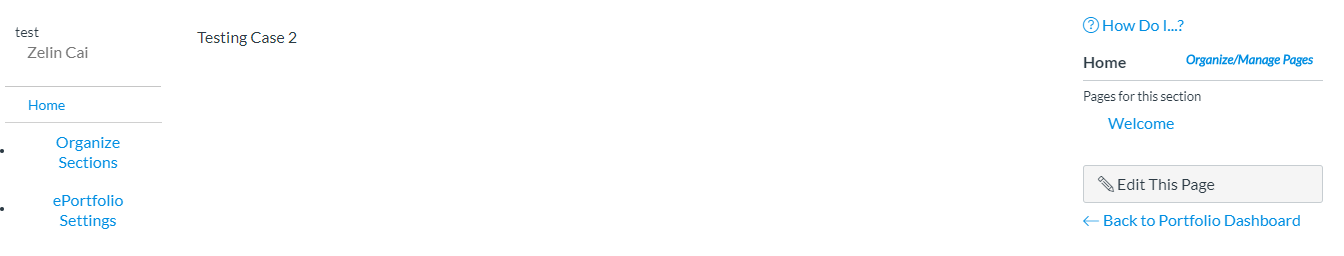
\includegraphics[width=\textwidth]{screenshots/tc12-actual-output.png}}
	\caption{TC-12 actual output}
\end{figure}
\pagebreak
\begin{figure}[h!]
	\centerline{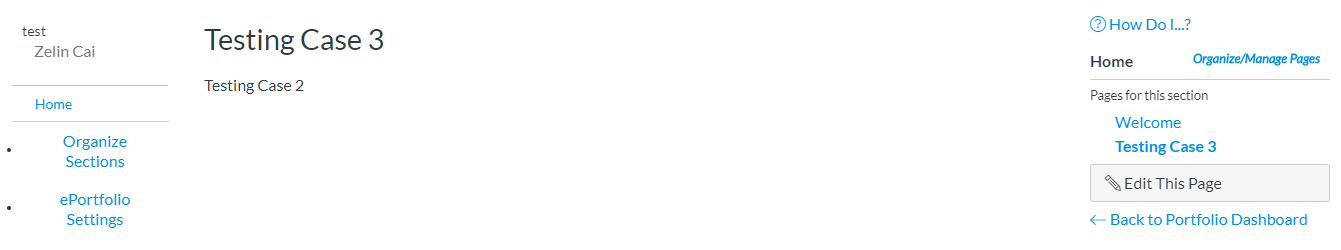
\includegraphics[width=\textwidth]{screenshots/tc13-actual-output.png}}
	\caption{TC-13 actual output}
\end{figure}
\begin{figure}[h!]
	\centerline{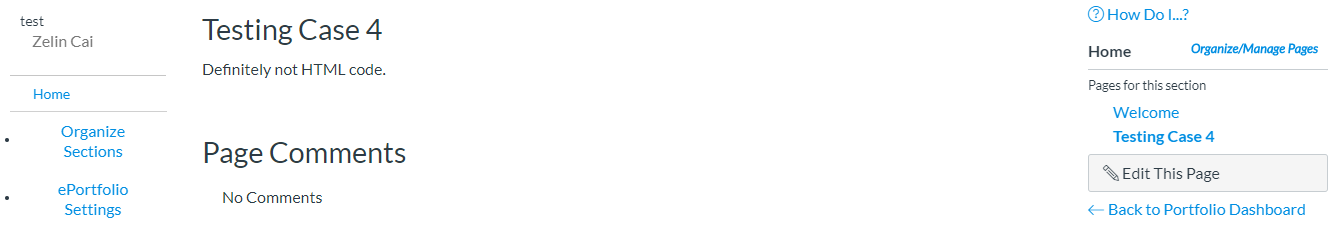
\includegraphics[width=\textwidth]{screenshots/tc14-actual-output.png}}
	\caption{TC-14 actual output}
\end{figure}
\begin{figure}[h!]
	\centerline{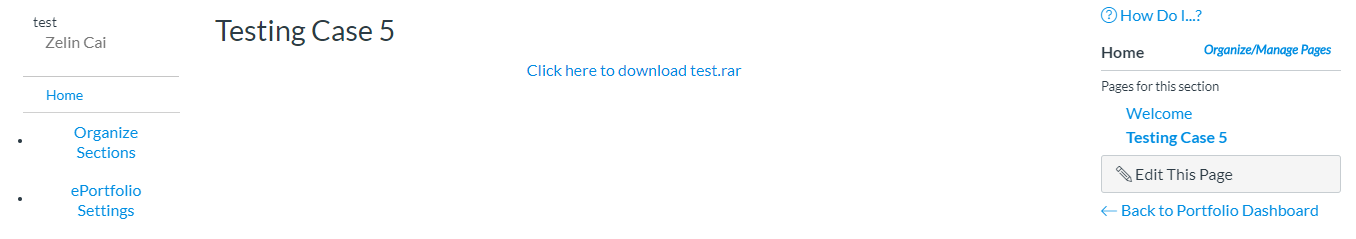
\includegraphics[width=\textwidth]{screenshots/tc15-actual-output.png}}
	\caption{TC-15 actual output}
\end{figure}

\newpage
\section{Files - File Management}
\subsection{Input Domain}
The "Files" feature on Canvas encompasses several different subfeatures. The subfeatures we will focus on are file upload, folder creation, file renaming, file deletion, and folder deletion.

\subsubsection{File Upload}
For file upload, the input domain is a file of any type. 

\subsubsection{Folder Creation}
For folder creation, the input domain is a string representing the folder name.

\subsubsection{File Renaming}
For file renaming, the input domain includes a file specified via the UI, a string representing the new filename, and a UI input for confirming or discarding the change.

\subsubsection{File Deletion}
For file deletion, the input domain includes a file specified via the UI, and a UI input for confirming deletion.

\subsubsection{Folder Deletion}
For file deletion, the input domain includes a folder specified via the UI, and a UI input for confirming deletion.

\begin{figure}[h!]
	\centerline{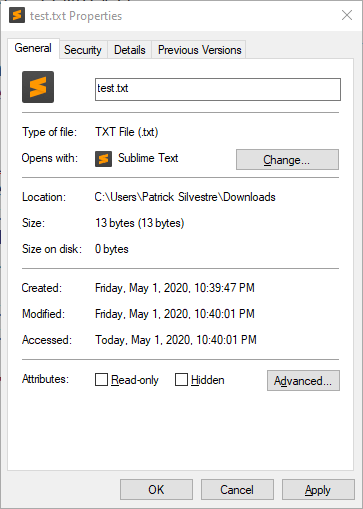
\includegraphics[width=8cm]{screenshots/file-test-file.png}}
	\caption{File to be used in applicable "Files" tests.}
\end{figure}

\newpage
\subsection{Test Cases}
\begin{table}[h!]
\begin{tabularx}{\textwidth}{lXXXl}
\toprule
TC \# &
  Input &
  Expected Output &
  Actual Output &
  Tess Pass/Fail \\ \midrule
16 &
  \begin{itemize}
    \item{UI: click "Upload" button}
    \item{file: \texttt{test.txt}}
  \end{itemize} &
   Canvas displays the uploaded file. &
   See figure 23. &
   Pass \\ \midrule
17 &
  \begin{itemize}
    \item{folder name: test}
  \end{itemize} &
   Canvas displays the created folder. &
   See figure 24. &
   Pass \\ \midrule
18 &
  \begin{itemize}
    \item{specified file: \texttt{test.txt}}
    \item{UI: click hamburger (option) menu for specified file}
    \item{UI: click rename option}
    \item{new filename: \texttt{abcd.txt}}
    \item{UI: click checkmark (confirm change)}
  \end{itemize} &
   Canvas displays the renamed file. &
   See figure 25. &
   Pass \\ \midrule
19 &
  \begin{itemize}
    \item{specified file: \texttt{abcd.txt}}
    \item{UI: click hamburger (option) menu for specified file}
    \item{UI: click delete option}
    \item{UI: click "Ok" button}
  \end{itemize} &
   Canvas accurately reflects deletion of file. &
   See figure 26. &
   Pass \\ \midrule
20 &
  \begin{itemize}
    \item{specified folder: \texttt{test}}
    \item{UI: click hamburger (option) menu for specified folder}
    \item{UI: click delete option}
    \item{UI: click "Ok" button}
  \end{itemize} &
   Canvas accurately reflects deletion of folder. &
   See figure 27. &
   Pass \\ \bottomrule
\end{tabularx}
\end{table}

\newpage
\begin{figure}[h!]
	\centerline{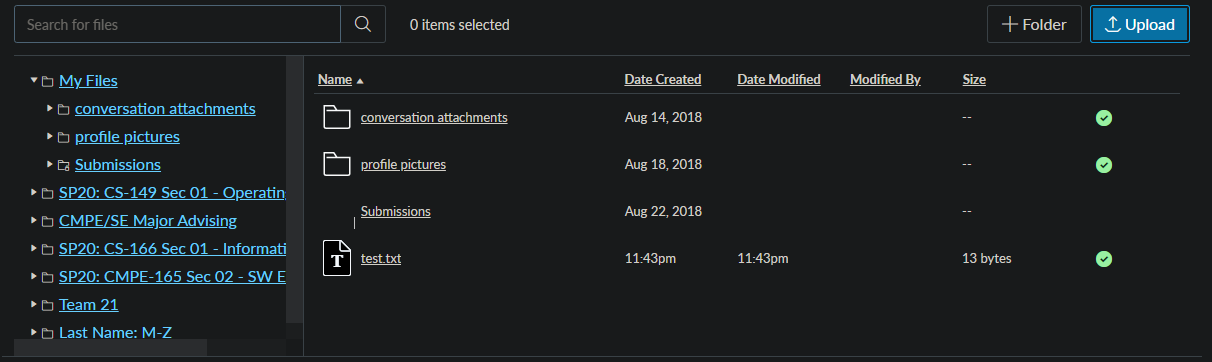
\includegraphics[width=\textwidth]{screenshots/tc16-actual-output.png}}
	\caption{TC-16 actual output}
\end{figure}
\begin{figure}[h!]
	\centerline{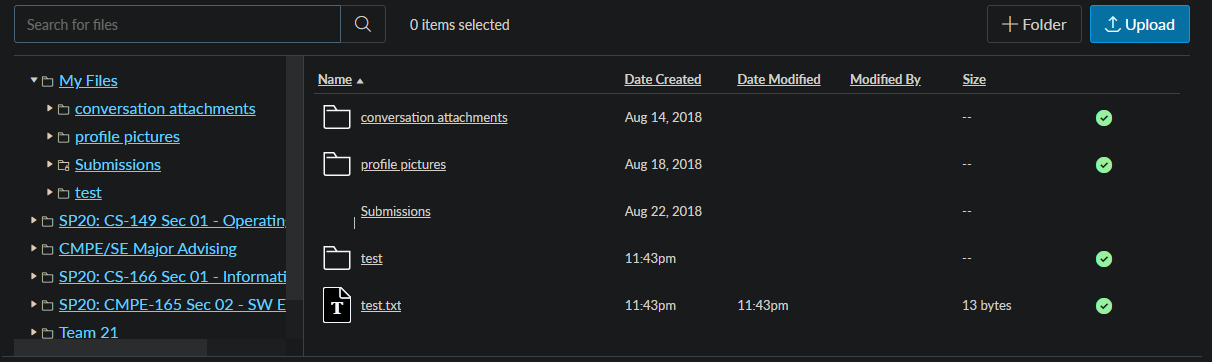
\includegraphics[width=\textwidth]{screenshots/tc17-actual-output.png}}
	\caption{TC-17 actual output}
\end{figure}
\begin{figure}[h!]
	\centerline{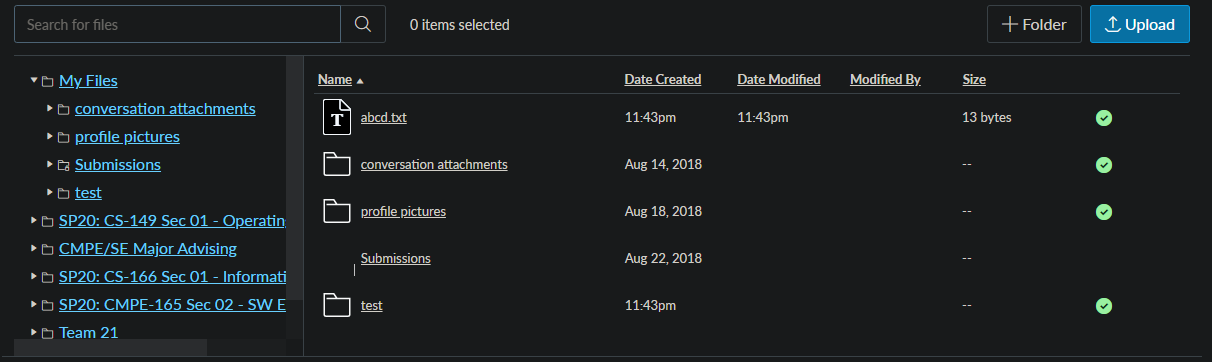
\includegraphics[width=\textwidth]{screenshots/tc18-actual-output.png}}
	\caption{TC-18 actual output}
\end{figure}
\pagebreak
\begin{figure}[h!]
	\centerline{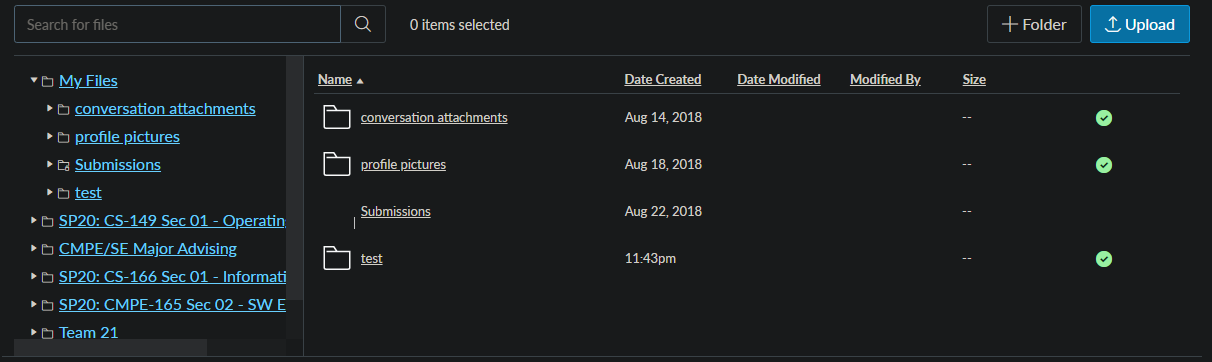
\includegraphics[width=\textwidth]{screenshots/tc19-actual-output.png}}
	\caption{TC-19 actual output}
\end{figure}
\begin{figure}[h!]
	\centerline{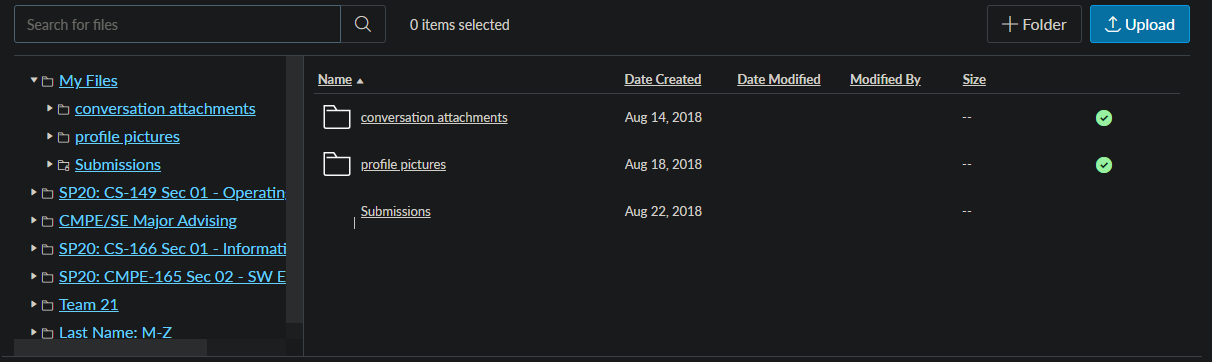
\includegraphics[width=\textwidth]{screenshots/tc20-actual-output.png}}
	\caption{TC-20 actual output}
\end{figure}
\end{document}